\section{Accelerating GaLore with Natural Gradients}

\subsection{Next Token Prediction}

Generative LLMs are trained to predict the next token in a sequence based solely on the previously observed tokens. This "causal" approach respects the temporal order of language, ensuring that the model's predictions at any point depend only on past and not future inputs.

Given a sequence of tokens \( x = (x_1, x_2, \dots, x_T) \), the objective is to maximize the likelihood of a sequence by decomposing it into a product of conditional probabilities:

\begin{eqnarray}
\text{Prob}_{\mathbf{\theta}}(x) = \prod_{t=1}^T \text{Prob}_{\mathbf{\theta}}(x_t \mid x_{<t})
\end{eqnarray}

where \( x_{<t} = (x_1, x_2, \dots, x_{t-1}) \) represents all tokens before position \( t \) and \( \text{Prob}_{\mathbf{\theta}}(x_t \mid x_{<t}) \) is the probability of the next token given all previous tokens and the parameter \( \mathbf{\theta} \in \mathbb{R}^{n \times m} \).

This is equivalent to minimizing the Negative Log-Likelihood (NLL) of the observed sequences, which is the cross-entropy loss between the predicted probability distribution and the actual next token:

\begin{eqnarray}
\Phi(\mathbf{\theta}) = -\sum_{t=1}^T \log \text{Prob}_{\mathbf{\theta}}(x_t \mid x_{<t})
\label{eq:cross_entropy_loss}
\end{eqnarray}

This loss penalizes the model more when it assigns lower probabilities to the correct next token. By minimizing this loss, the model learns to assign higher probabilities to appropriate continuations of text. However, the loss is non-convex and high-dimensional, for LLMs the dataset is also massive, making the optimization problem very challenging.

\subsection{Low-Rank Gradient Descent}

Stochastic gradient descent algorithms are iterative, where each step aims to find the optimal update direction that minimizes the loss function locally. Now in the case of GaLore, the update direction is restricted to the affine subspace \(\mathbf{u}_{k} \in {\mathbf{\theta}_{k}} + \text{Range} \left(\mathbf{P}_{k}\right)\). Here \(\mathbf{P}_{k} \in \mathbb{R}^{n \times r}\) is the left projection matrix, calculated using the compact SVD decomposition of the gradient matrix \(\nabla_{\mathbf{\theta}} \Phi(\mathbf{\theta}_{k}) = \mathbf{P}_{k} \Sigma \mathbf{Q}_{k}^{T}\).

Then, the local neighborhood around this update can be defined using the Taylor series expansion \citep{lin2022randomized}:

\begin{eqnarray}
\Phi(\mathbf{\theta}_{k} + \mathbf{P}_{k} \mathbf{u}_{k}) \approx \Phi(\mathbf{\theta}_{k}) + \mathbf{g}_{k}^{T}\mathbf{u}_{k} + \frac{1}{2} \mathbf{u}_{k}^{T} \mathbf{H}_{k}  \mathbf{u}_{k}
\label{eq:taylor_series_expansion}
\end{eqnarray}

where \(\mathbf{g}_{k} = \mathbf{P}_{k}^{T}\nabla_{\mathbf{\theta}} \Phi(\mathbf{\theta}_{k})\) is the low rank projected gradient and \(\mathbf{H_{k}} = \mathbf{P}_{k}^{T}\nabla^2_{\mathbf{\theta}} \Phi(\mathbf{\theta}) \mathbf{P}_{k}\) is the Hessian matrix.

However, the Hessian matrix \(\mathbf{H}_{k}\) is often computationally expensive to compute and store, especially for large-scale language models (LLMs) with billions of parameters. Fortunately, precisely under the condition that the loss function can be represented in terms of KL divergence between the actual and approximated distributions [\ref{eq:cross_entropy_loss}], then \(\mathbf{H_{k}}\) can be approximated by the FIM. The FIM is defined as the expectation of the Hessian of the negative log-likelihood w.r.t. the data distribution:

\begin{eqnarray}
\mathbf{F}_{k} = \mathbb{E}_{x \sim p_{\text{data}}} \left[ \mathbf{H}_{k} \right]
\end{eqnarray}

The FIM captures the curvature of the loss landscape and provides a natural metric for the optimization process. Hence, it can better adjust parameter updates according to the geometry of the parameter space. However, as the theoretical data distribution is unknown, in practice, we need to estimate it using the empirical FIM \citep{martensNewPerspectiveNatural2014} defined by:

\begin{eqnarray}
\mathbf{\hat{F}}_{k} = \frac{1}{h} \sum_{k=1}^{h} \mathbf{g_{k}} \mathbf{g_{k}}^{T}
\end{eqnarray}

where \(h\) is the history of gradients from past batches we would like to consider. Then, the optimal direction \(\mathbf{u}_{k}^{*}\), which minimizes the loss in this local neighborhood, is given by (cite Fuji et al. paper):

\begin{eqnarray}
\mathbf{u}_{k}^{*} &=& \mathbf{\hat{F}}_{k}^{-1} \mathbf{g}_{k}
\label{eq:optimal_direction}
\end{eqnarray}

This leads to the optimal gradient descent update step:

\begin{eqnarray}
\mathbf{\theta}_{k+1} = \mathbf{\theta}_{k} - \eta \mathbf{P}_{k} \mathbf{u}_{k}^{*}
\label{eq:gradient_descent_update}
\end{eqnarray}

for some learning rate \(\eta\).

Many popular stochastic optimization algorithms approximate the diagonal of the empirical FIM using second-moment estimates of the gradient \(\mathbf{g}_{k}\), which when added with Polyak style parameter averaging (i.e., momentum), asymptotically achieve the optimal Fisher efficient convergence rate \citep{martens2020new}.

For instance, in the case of Adam \citep{kingmaAdamMethodStochastic2014}, the optimal update step is approximated by including the momentum term \(\mathbf{m}_{k} \in \mathbb{R}^{r\times m}\) and the learning rate \(\eta\) is scaled by the square root of the second moment estimate \(\mathbf{v}_{k} \in \mathbb{R}^{r\times m}\). With all operations being elementwise, the update direction becomes:

\begin{eqnarray}
    \mathbf{m}_{k} &=& \beta_{1} \mathbf{m}_{k-1} + (1-\beta_{1}) \mathbf{g}_{k} \\
    \mathbf{v}_{k} &=& \beta_{2} \mathbf{v}_{k-1} + (1-\beta_2) \mathbf{g}^{2}_{k}  \\
    \mathbf{u_{k}^{*}} &=& \mathbf{m}_{k} / \sqrt{\mathbf{v}_{k} + \epsilon}
    \label{eq:adam_update}
\end{eqnarray}

This update, when applied to [\ref{eq:gradient_descent_update}], gives the GaLore optimization algorithm, which is memory efficient as it only requires storing the projection matrix and the costly optimizer states \(\left(g_{k}, m_{k}, v_{k}\right)\) are now significantly reduced by a factor of \(\frac{n}{r}\), where the rank \(r\), can be chosen based on the tradeoff between memory limitations and performance requirements.

\subsection{\lowrank and Fisher Efficiency}

Despite clear advantages, the performance of GaLore is not on par with AdamW \citep{loshchilov2017decoupled} optimization on the original space. To bridge this gap, we propose \textit{\lowrank}, which uses the full empirical FIM, thereby incorporating the missing second-order interaction information in the optimization process.

As we now argue, this leads to a much more favorable dependence on the starting point, which means that the optimizer can make much more progress given a limited iteration budget. Further, when using a decaying learning rate schedule like with AdamW \citep{loshchilov2017decoupled}, the asymptotic convergence rate can be faster \citep{martens2020new} by a significantly large constant factor.

Natural gradient descent is known \citep{martens2020new} to be Fisher efficient, precisely for our loss function [\ref{eq:cross_entropy_loss}]. Fisher efficiency means that the natural gradient estimator asymptotically achieves the lowest possible variance among all unbiased gradient estimators.

For \textit{\lowrank}, the gradient descent update [\ref{eq:gradient_descent_update}] leads to a sequence of estimates \( \mathbf{\theta}_{k} \) whose variance satisfies \citep{amariNaturalGradientWorks1998}:

\begin{eqnarray}
\text{Var}[\mathbf{\theta}_{k}] = \frac{1}{mk} \mathbf{F}_{k}^{-1}(\mathbf{\theta}_{k}^*) + \mathcal{O}\left(\frac{1}{k^2}\right)
\label{eq:variance_reduction}
\end{eqnarray}

which is asymptotically the smallest possible variance matrix satisfying the Cramér-Rao lower bound, that any unbiased estimator computed from \(mk\) training samples can have, with \(m\) being the batch size.

Here, \(\mathbf{\theta}_{k}^*\) is the local optimum in the neighborhood defined by the Taylor series expansion [\ref{eq:taylor_series_expansion}] around the update direction. This is an important caveat, as the guarantee is only for local convergence in a convex neighborhood. The loss function is non-convex, so the property can not be stated to hold for the global optimum.

The result also relies on the computation of the exact FIM \( \mathbf{F}_{k}(\mathbf{\theta}_{k}) \) using the entire data distribution, which is not practical. The Fisher efficiency guarantee is, however, only approximately satisfied when using the empirical FIM \(\mathbf{\hat{F}_{k}}\) instead. Nevertheless, we still get a variance reduction in the gradient estimates, leading to faster convergence and better optimization performance in the early stages of training large-scale models, making it especially valuable for training with a limited iteration budget.

Further, incorporating second-order information through the empirical FIM allows the optimizer to account for the curvature of the loss landscape, enabling natural gradient descent to take more informed steps than standard gradient descent, potentially escaping flat regions or navigating steep ravines more effectively.

In \citep{martens2020new}, it was shown that the expected update direction can be expressed as a sum of two terms, one that scales as \(\mathcal{O}(1/k)\), which is independent of the starting point and another that scales as \(\mathcal{O}(1/k^2)\), which is dependent on the starting point. If momentum is applied to the gradient estimator, the first term becomes independent of the choice of FIM estimator, thereby not leading to any asymptotic improvements. However, regularizing with the empirical FIM estimate can significantly reduce the constant factor associated with the starting-point-dependent second term. This leads to practical performance gains in finite iteration regimes (although negligible for large \(k\)).

Finally, the Fisher efficiency result also assumes that the model can perfectly capture the data distribution, a condition known as \emph{realizability}. However, with the growing size of LLMs, this assumption is likely to hold, thereby satisfying the conditions for the guarantee. Therefore, especially in low-resource settings, \textit{\lowrank} can be a promising approach for training LLMs under memory constraints.

\subsection{Natural Gradient Transform}

Our \textit{\lowrank} algorithm is designed to efficiently apply the inverse empirical FIM to low-rank gradients using Woodbury's Identity. Most of the steps in the algorithm are similar to GaLore \citep{zhao2024galore}, with the critical difference being the incorporation of the natural gradient transform.

% 



\definecolor{cus_color}{rgb}{22, 96, 55}


\makeatletter
\newcommand{\removelatexerror}{\let\@latex@error\@gobble}
\makeatother


\begin{figure}[!t]
\centering
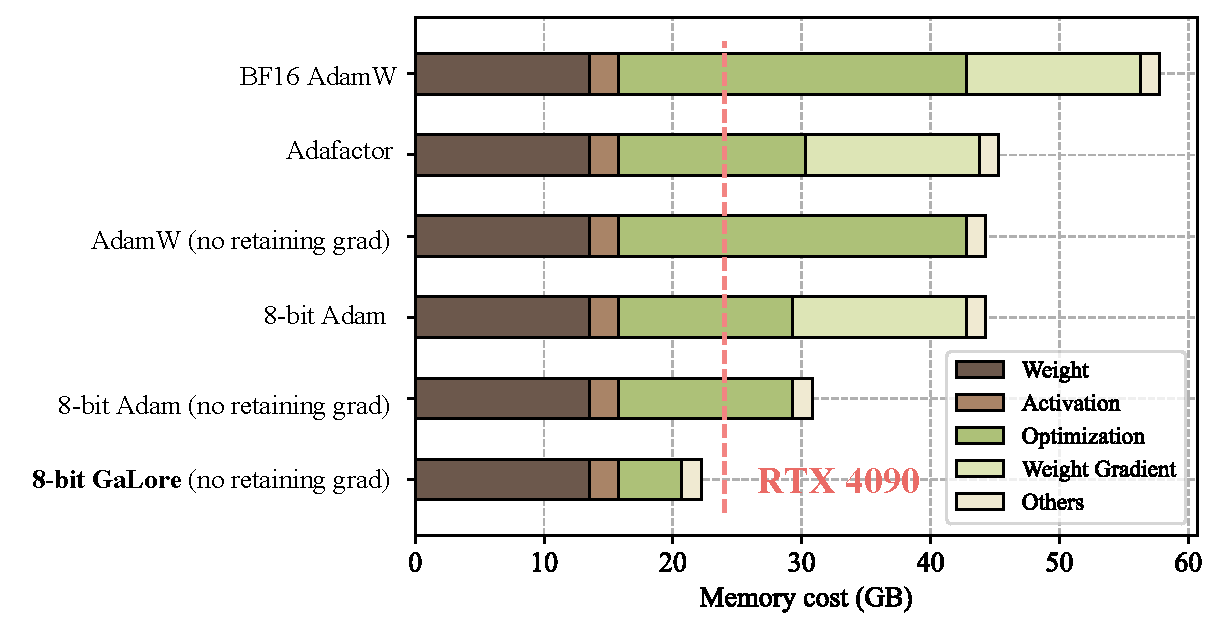
\includegraphics[width=1\columnwidth]{figures/files/memory_breakdown.pdf}
\vskip -0.11in
\caption{\small{Estimated memory consumption of pre-training a LLaMA 7B model with a token batch size of 256 on a single device, without activation checkpointing and memory offloading\protect\footnotemark[2]. Details refer to Section~\ref{sec:memory_measure}.}}
\label{fig:memory_breakdown} 
\vskip -0.15in
\end{figure}
\footnotetext[1]{The calculation is based on LLaMA architecture, BF16 numerical format, and maximum sequence length of 2048.}
\footnotetext[2]{In the figure, ``no retaining grad'' denotes the application of per-layer weight update to reduce memory consumption of storing weight gradient \citep{lvFullParameterFinetuning2023}.}
\SetAlFnt{\fontsize{8pt}{9pt}\selectfont}
\SetAlCapFnt{\fontsize{8pt}{9pt}\selectfont}
\begin{algorithm}[t]
    \SetAlgoLined
        \PyCode{for weight in model.parameters():} \\
        \Indp   %
            \PyCode{grad = weight.grad} \\ 
            \PyComment{original space -> compact space} \\
            \PyCode{lor\_grad = \textbf{project}(grad)} \\
            \PyComment{update by Adam, Adafactor, etc.} \\
            \PyCode{lor\_update = \textbf{update}(lor\_grad)} \\
            \PyComment{compact space -> original space} \\
            \PyCode{update = \textbf{project\_back}(lor\_update)} \\
            \PyCode{weight.data += update} \\
        \Indm %
    \caption{\fontsize{8pt}{9pt}\selectfont{\lowrank{}, PyTorch-like}}
    \label{alg:code_box}
\end{algorithm}


In order to implement the natural gradient transform, we compute the inverse of the empirical FIM and apply it to the gradient \(\mathbf{g_{k}}\) using Woodbury's Identity, which allows us to efficiently compute the inverse of a matrix of the form \(A + UBU^T\). Woodbury's Identity states that:

\begin{eqnarray}
(A + UBU^T)^{-1} = A^{-1} - A^{-1}U(B^{-1} + U^TA^{-1}U)^{-1}U^TA^{-1}
\end{eqnarray}

Now, if we choose \(\mathbf{\hat{F}}_{k} = \lambda I + GG^{T}\), \(A = \lambda I\), \(U = G\), and \(B = I\), where \(G = [\operatorname{vec}(\mathbf{g}_{k}), \operatorname{vec}(\mathbf{g}_{k-1}),\ldots, \operatorname{vec}(\mathbf{g}_{k-s})]\) is the stacked gradient matrix over the past \(s\) gradients and \(\lambda\) is a small constant for Tikhonov regularization, then, the inverse of the empirical FIM applied to the gradient \(\mathbf{g_{k}}\) i.e. the natural gradient \(\mathbf{\tilde{g}}_{k} = \mathbf{\hat{F}}_{k}^{-1}\mathbf{g_{k}}\) can be calculated as:

\begin{eqnarray}
 \mathbf{\tilde{g}}_{k} = \frac{1}{\lambda}\mathbf{g_{k}} - \frac{1}{\lambda}G\left(\lambda I + G^{T}G\right)^{-1}G^{T}\mathbf{g_{k}}
\end{eqnarray}

To compute the above formula efficiently, let \(S = I + \frac{1}{\lambda}G^{T}G \in \mathbb{R}^{s\times s}\) and \(y = G^T\mathbf{g_{k}}\). Cholesky decomposition is used to solve for \(z\) in
\begin{eqnarray}
S z = y
\end{eqnarray}
which requires only \(\mathcal{O}(s^2)\) time. Then, the final natural gradient estimate can be computed using only matrix-vector products, which is very memory efficient:
\begin{eqnarray}
 \mathbf{\tilde{g}}_{k} = \frac{1}{\lambda}\mathbf{g_{k}} - \frac{1}{\lambda^{2}}Gz
\end{eqnarray}
This natural gradient estimate \(\mathbf{\tilde{g}}_{k}\) can then be sent to the Adam optimizer [\ref{eq:adam_update}], and the model parameters the same way as in GaLore.